\documentclass[pdftex,12pt,a4paper]{report}
\usepackage{dbstmpl}

% Hier die eigenen Daten eintragen
\global\arbeit{Bachelor Thesis}
\global\titel{Optical Character Recognition for Labels Using Deep Learning}
\global\bearbeiter{Johannes Reichle}
\global\matrikel{04797218}
\global\betreuer{Prof.\ Dr.\ Rainer Schmidt}
\global\aufgabensteller{Random Ltd.}
\global\abgabetermin{XX.XX.2022}
\global\ort{Munich}
\global\fach{Information Systems and Management}

\begin{document}

\deckblatt
\erklaerung

\erklaerung

\begin{abstract}
    Here abstract for \the\arbeit.

    \vspace*{150px}

    {
        \noindent
        \textbf{Keywords:} Deep Learning, Optical Character Recognition, Scene Text Recognition,
        Literature Review
    }
\end{abstract}

\tableofcontents
% FIXME: seitenzahlen

\listoffigures

% delete group thing to have tables on new page
\begingroup
    \let\clearpage\relax
    \listoftables
\endgroup

\chapter*{Abbreviations}
\addcontentsline{toc}{chapter}{Abbreviations}
\printacronyms[heading=none]


\tableofcontents

\listoffigures

% delete group thing to have tables on new page
\begingroup
    \let\clearpage\relax
    \listoftables
\endgroup

\chapter*{Abbreviations}
\addcontentsline{toc}{chapter}{Abbreviations}
\printacronyms[heading=none]

\chapter{Introduction}\label{ch:intro}

% TODO: replace Computer Vision with OCR -> make sure it's ok with citations
\section{Motivation}
Nowadays it is hard to find a business process that doesn't use software for improvement.
Various technologies come to be valued because of this.
A recent trend is to use Deep Learning for types of problems that range from self driving
cars to medical diagnosis~\cite{balas_handbook_2019}.
Deep Learning is a powerful technology based on Artificial Neural Networks where data is processed
in multiple layers to extract features and solve a given problem~\cite{shrestha_review_2019}.
One area where this is especially helpful is the field of Computer Vision.
Deep Learning for Computer Vision has only caught on in the recent years as the big computational
cost has been met by the improvement in computer hardware~\cite{ponti_everything_2017}.
Computer vision deals with extracting information from photos.
This includes tasks like recognizing faces or reading text~\cite{prince_computer_2012}.
Applying Deep Learning to extract equipment labels from photos fits right into this crease of
applying technology for making daily problems more efficient.
Combining the two fields to create value and learning about the underlying theoretical foundations
and inner workings is the motivating factor of this work.

\section{Problem description}\label{se:problem}
% TODO: add costs
% TODO: cut down this part -> put into EDA part
% TODO: define requirements better
Motivated by the wide success of Deep Learning concerning Computer Vision,
the objective of this work is to implement and train a Deep Learning model that can extract
equipment names from photos taken of name plates.

When determining whether automisation is an improvement four aspects have to be examined.
These are time, costs, quality and flexibility.
The aspects build a quadrangle that is based on the optimizing trade-off between the
factors~\cite{dumas_fundamentals_2013}.

Without software supporting the task of reading the name of the picture  and typing it into
the system, can take long seconds, whereas a trained Deep Learning model could complete the task
in a mere instant.
Therefor automisation via Deep Learning should improve the efficiency of the process when compared to
manually reading and typing the information off the image.

Training costs for a Deep Learning model are very high due to the computing intensive
backpropagation algorithm that tunes the network to the data.
But the usage cost is low.
For manual labor the opposite is the case as training a person to type in a label is done quickly
and labor costs are high in comparison to the expenses for running the model.

Both Deep Learning models and human labor are not 100\% accurate.
It is human to make mistakes and because Deep Learning is trained only trained on a specific set
of data it makes sense that not all predictions can be correct as there can always be outliers in
the data. % TODO: find source
The question is whether the model can be as accurate or even better than its human counterpart.
This is especially interesting when it is applied in the real world where it might have to do good
in subpar situations.
An example is bad image quality.

Flexibility is concerned with how well a process can adjust to changing requirements.
A set of new equipment names that have to be included can pose a problem to a Deep Learning model
because it is not trained for the new data.
A human on the other hand should not have any problems in this regard.

The main concern for the solution's efficacy is whether it is accurate enough.
Therefor this work focuses on this aspect in particular.

\section{Methodology}

The goal of this work is to implement and train a Deep Learning model to read in labels from photos.
The emerging artifact can be used to solve the problem detailed in~\ref{se:problem}.
The expository instantiation is helpful to gain more understanding the artifact as it is common
in design science.
In particular this is justificatory knowledge on the design on the Deep Learning model and
Machine Learning way of approaching problems.
This is important in order to apply it and to optimize existing research to the specific problem.

The methodology is based on action research~\cite{johannesson_introduction_2021}.
It constists of a cycle of five phases: Diagnosis, Planning, Intervention, Evaluation, Reflection.
% TODO: add how I get data
The first cycle will entail an exploratory data analysis which corresponds to the Diagnosis part.
Here it is important to recognize main characteristics of the images and to find outliers
and other potential problems~\cite{cox_translating_2017}.
The research is then extended to existing practical solutions for similar practical problems as
well as proposed architectures from academic research.
Theoretical knowledge about the models as well as practical information about results for
similar problems contribute to the discussion about which approach is the most promissing.
Combining architectures is also a viable possibility to solve the given problem.
This concludes the Planning phase and will lead to a model exaptation that evolves to be the
artifact at the center of this thesis.
The next step is implementing and training the chosen approach which.
Evaluation for of the current model follows.
Storing and analyzing results of training and cross validation as well as visualizing the training
progress is an important part of this.
In the Reflection stage it is decided whether a new cycle should be carried out.

From the second cycle on the first three phases change as there already is a model that is to be
improved.
This time the Diagnosis phase entails asking questions about the existing model: What worked?
Why did it work/not work? What needs to change?
Changes are planned and implemented accordingly.
The Evaluation and Reflection phases are not changing in the second cycle thus closing the loop.
The incremental adjustments to the model are made in order to improve the accuracy.
This includes possibly adjusting the architecture, hyperparameter tuning and preprocessing approaches
like image compression.

\section{Expected results and outlook}
The research into the theoretical foundation of Deep Learning and into possible approaches leads
to a strong understanding of the underlying technology.
This is helpful to produce a comparison of approaches that is based on theoretical as well as
practical knowledge.
The goal is to find out which approach work best for the chosen practical problem and why that is the
case.
Implementation and training of the most promissing one is yielding the artifact this work revolves
around.
The process of optimization not only improves the solution to the problem (see~\ref{se:problem}) but
is also used to learn more about the implemented approach.

Integrating the artifact into the business process is not an issue that is discussed in
this work.
Nor will model feedback and over time iteration be part.

The intendet structure of the thesis with dependencies between chapters can be found in
figure~\ref{fig:chapters}.

\begin{figure}[ht]
    \centering
    \includegraphics[width=1.0\textwidth]{img/Chapter.drawio.png}
    \caption{Chapters with subchapters and dependencies\label{fig:chapters}}
\end{figure}

\chapter{Theoretical Foundation}\label{ch:theoretical}
This chapter succinctly describes principles which build the foundation for later chapters.
Only the most relevant topics are touched upon, as the details are explained in later chapters.
The mathematics that makes the techniques possible is not explained in depths.

\section{Machine Learning}
In order to grasp \ac{DL}, a solid understanding of \ac{ML} has to be developed
first~\citep{goodfellow_deep_2016}.
This is because \ac{DL} is a subfield of \ac{ML}~\citep{chauhan_review_2018}.
The most well known definition for \ac{ML} comes from~\cite{mitchell_machine_1997}:
`A computer program is said to learn from experience $E$ with respect to some class of tasks $T$
and performance measure $P$, improves with experience $E$'.

% XXX: explain difference: model - algorithm
The task that the \ac{MLS} learns to perform, can range from approximating a function
(e.g.\ regression --- $f:\R^n \rightarrow \R$, classification ---
$f:\R^n \rightarrow \{1,\ldots,k\}$) to optaining a different representation for the data that
has beneficial properties for further processing but preserves as much information as possible
(e.g.\ PCA for compression)~\citep{goodfellow_deep_2016}.
Note that the learning itself is not the task but merely the process of improving on performing the
task~\citep{goodfellow_deep_2016}.
One of the most well known \ac{ML} algorithms is Linear Regression.
In the following the algorithm is used as an example for explaining \ac{ML} principles.
As the name implies, Linear Regression is used to predict a value $\hat{y}$ given the input vector
$\x\in\R^n$ which is made up of the features $x_i$.
The goal is to approximate the ground truth $y$.
Linear is derived from the underlying model shown in Equation~\ref{eq:linReg}:
\begin{equation}\label{eq:linReg}
    f(\x;\w,b) = \w^{T} \cdot \x + b = \sum_{i=1}^{n} w_i x_i + b = \hat{y}
\end{equation}
The scalar product of the weights $\w\in\R^n$ and \x\ is added to the bias term $b\in\R$.
Both $\w,b$ are parameters that are learned by the model in order to optimize the
approximation~\citep{goodfellow_deep_2016}.
% FIXME: here figure with linear regression

The performance of a model measures how well the task can be completed.
Depending on the task of the \ac{MLS}, different quantitative measures are used.
The metric Mean Squared Error (see Equation~\ref{eq:mse}) can be used for Linear Regression.
\begin{equation}\label{eq:mse}
    MSE =\frac{1}{m}\norm{{(\hat{\textbf{y}} - \textbf{y})}}^2
        =\frac{1}{m}\sum_{i=1}^m {((\w^T \x^{(i)} + b) - \yti)}^2
\end{equation}
Here $m$ denotes the number of examples $\X$ with the associated targets \y, used to calculate
the error~\citep{geron_hands-machine_2017,goodfellow_deep_2016}.
The goal is to minimize the generalization error which measures the expected performance on
previously unseen input~\citep{geron_hands-machine_2017}.
For this the test set is used, once the model has been trained.
The test set is a part of the available data~\citep{geron_hands-machine_2017, goodfellow_deep_2016}.
The generalization error can be divided into three components.
The bias error arises from simplifying assumptions for the model, the variance error measures the
variation in the model outcome depending on the data used for training.
Both these errors are influenced by the model's capacity which is why the relationship between them
is call the Bias/Variance tradeoff.
Lastly the irreducible error stems from not having measured all data as well as the variation
in real data and cannot be
reduced~\citep{ashmore_assuring_2021, james_introduction_2013,geron_hands-machine_2017}.

The experience part of \ac{ML} depicts the process where the algorithm is `experiencing' the training
dataset $\Xt$ and is learning important properties of the dataset.
In general there are two paradigms for training: supervised and
unsupervised~\citep{goodfellow_deep_2016}.
Linear Regression is an example for supervised learning, as the model is approximating the target
value $\yti$\ for the associated input $\xti$~\citep{alzubi_machine_2018,goodfellow_deep_2016}.
For unsupervised learning on the other hand the algorithm is not directed to predict a target
value but to learn properties about the data and to leverage them for representation tasks
like compressing or denoising the data~\citep{goodfellow_deep_2016}.
The important difference between the paradigms is that the unsupervised learning algorithm does
not use a target value, there's no ground truth
value~\citep{goodfellow_deep_2016,geron_hands-machine_2017}.
In most cases training can be described as an optimization problem, i.e.\ as minimizing a
function --- the so called objective or loss function~\citep{goodfellow_deep_2016}.
The MSE introduced earlier can be used for Linear Regression (see Equation~\ref{eq:mseOpt}).
This objective function has properties which make it suitable for models which have linear
output~\citep{goodfellow_deep_2016}.
\begin{equation}\label{eq:mseOpt}
    \min_{\w,b} MSE(\w,b)
\end{equation}
Note that for minimization the MSE is a function of $\w,b$ and not of $\x$, in terms of
predicting a value the MSE is a function of $\x$ parametrized by $\w,b$.
In Equation~\ref{eq:linReg} \w,$b$ are parameters that have to be learned in order to minimize
the generalization error~\citep{james_introduction_2013,geron_hands-machine_2017}.
For other tasks such as binary classification, the metric (e.g. $F_1$-Score) and the
objective function (binary cross entropy loss) are different~\citep{geron_hands-machine_2017,
ho_real-world-weight_2020}.
% FIXME: simple gradient descent figure / learning process graphic
For optimization the \ac{GD} algorithm is prevalent, especially in the subfield of \ac{DL}.
As the name suggests, the gradient is used to iteratively update the parameters $\w,b$ to arrive
at a minimum of the objective function (see Equation~\ref{eq:gradDescW}
and~\ref{eq:gradDescb})~\citep{geron_hands-machine_2017}.
\begin{equation}\label{eq:gradDescW}
    \w \leftarrow \w - \epsilon \cdot \nabla_{\w} MSE(\w,b) = \w-\frac{2\epsilon}{m}\Xt^T (\Xt\w+b-\y)
\end{equation}
\begin{equation}\label{eq:gradDescb}
    b \leftarrow b - \epsilon \cdot \frac{\delta}{\delta b} MSE(\w,b) = b-\frac{2\epsilon}{m}(\Xt\w+b-y)
\end{equation}
The learning rate constant $\epsilon$ can be adjusted to speed up or slow down the `steps' which
can have different effects on the convergence~\citep{goodfellow_deep_2016}.
There are more sophisticated variations of the \ac{GD} algorithm which are more suited for practical
application (e.g. RMSProp, Adam)~\citep{geron_hands-machine_2017}.
Note that the process minimizes the test error with the test set $\Xt$.
The effect on the generalization error depends on model capacity which is the space of functions
the model enables~\citep{goodfellow_deep_2016}.
Linear Regression has the capacity to fit to data with a linear relationship between features and
ground truth.
If the underlying relationship is more complicated, the model can only underfit the data (model
bias)~\citep{goodfellow_deep_2016}.
Polynomial Regression has more capacity for example.
Say the real relationship between features and ground truth now actually is linear;
the Polynomial Regression model can overfit for statistical outliers in the test set which is why
in this case the model with the lower capacity can achieve a lower generalization
error~\citep{geron_hands-machine_2017}.
Therefore, it is important to improve the bias/variance tradeoff.
% FIXME: graphic for underfitting/overfitting -> LinRegr - Under, PolRegr - Over / Fig 5.3 goodfellow

\section{Deep Learning}
approximate a function

` One of the main differences from traditional ma- chine learning (ML) methods is that DL
automatically learns how to represent data using multiple layers of abstraction [5], [6].
In traditional ML, a significant amount of work has to be spent on “feature engineering” to
build this representation manually, but this process can now be automated to a higher degree.
Having an automated and data-driven method for learning how to represent data improves both the
performance of the model and reduces requirements for manual feature engineering work
[7], [8].'~\citep{arpteg_software_2018}

\begin{enumerate}
    \item ANN / MLP % Node, Feedforward, Backpropagation / Optimization
        \begin{itemize}
            \item Architecture $\rightarrow$ Input, Hidden, Output
            \item Feedforward
            \item Optimization $\rightarrow$ Backpropagation, SGD, ADAM, \ldots
        \end{itemize}
    \item Regularization: L0,L1,L2, Dropout, Dropconnect
    \item important architectures
        \begin{itemize}
            \item CNN % layers --- convolutional, max-pooling
            \item RNN % recurrent layer
            \item transformer
            \item Specific foundation architectures for relevant approaches
        \end{itemize}
    \item transfer learning: reuse parameters from pretrained models\\
\end{enumerate}

\section{Optical Character Recognition}

\begin{enumerate}
    \item def
    \item little history
    \item need for \ac{STS}
    \item evaluation metric and matching prediction to ground truth
    \item common data sets
\end{enumerate}

\chapter{Problem analysis}\label{ch:problem}
This chapter entails an analysis of the problem which is the research question's foundation.
It is crucial, as the quality of requirements ultimately determines the quality of the overview and
subsequent analysis.

Requirements for a software system that involves \ac{ML} and thus \ac{DL} differs from
the traditional approach. The data-driven software components are not entirely defined by the
programmer but are influenced by data.
The system acts with dependency on the test data~\citep{siebert_construction_2021}.
This poses a challenge in determining requirements and measuring quality of
results~\citep{nakamichi_requirements-driven_2020}.
Instead of categorizing functional and non-functional requirements, like for traditional
software projects~\citep{zowghi_requirements_2014}, qualities that a \ac{MLS} must possess
are defined.

In the article~\cite{ashmore_assuring_2021} the qualities are identified and assigned to different
challenges in regards to working with \ac{MLS}: Development Challenges, Production Challenges,
Organizational Challenges.
Because the only the Model Selection substage of the lifecycle is performed, the challenges and their
qualities are not relevant for this thesis, as they concern the operational aspect of \acp{MLS}.

In~\cite{nakamichi_requirements-driven_2020,siebert_construction_2021} systematic approaches for
identification and documentation of qualities are detailed.
In \acp{MLS} various entities interact to in order to produce the desired functionality.
The paper~\cite{nakamichi_requirements-driven_2020} suggests that in order to adequately evaluate
the qualities, it is essential to not only consider the model but the entire \ac{MLS}.
These entities are data, model, environment,
system/infrastrucure~\citep{nakamichi_requirements-driven_2020, siebert_construction_2021}.
The article~\cite{siebert_construction_2021} differenciates between system and infrastrucure.
The infrastrucure represents given hardware and available libraries, whereas the system depicts
the software that surrounds the model in the runtime environment.
% TODO: explain entities: data, environment, model?
For this thesis the entities data and system cannot be regarded as given.
The entities environment and infrastrucure are only losely defined through the use case.
That is why the systematic approaches cannot be performed in the scope of this thesis.
For example~\cite{siebert_construction_2021} proposes to follow the systematic CRISP-DM approach of
identifying qualities.
It cannot be performed due to the lack of data and the other entities.
Instead many qualities that are highlighted by research that fit the problem are taken into account
along with two critical qualities (alphanumeric recognition, semantic retention) that are directly
derived from the use case.
When it comes to documenting the identified qualities,
both~\cite{nakamichi_requirements-driven_2020} and~\cite{siebert_construction_2021} define a meta
model for qualities that combines qualities with
measurement methods and values and assignes them to an entity of the \ac{MLS}.
The implementation and testing phase are not performed in the scope of this thesis and the
difficulty in assessing the performance ahead of those phases, prevents the evaluation
of measurements.
Additionally, experimental results from literature can only be compared as long as factors such as
hardware, platform, source code, configuration and dataset are uniform~\citep{arpteg_software_2018}.
This applies to studies that create an overview such as~\cite{chen_text_2021,long_scene_2021}.
These studies can only be regarded as guiding values because the performance for a specific dataset
cannot be predicted without testing on it~\cite{arpteg_software_2018}.
% TODO: ok like that? then compare relative to each other not absolute
That's why targets for measurements are not defined, as evaluation would only deliver a false
sense of certainty.

The problem can be depicted by a use case.
This use case sets the foundation for determining requirements for an
approach because qualities derive from the intended purpose of
use~\citep{siebert_construction_2021}.
For this thesis, the basic use case is as follows:
% TODO: where exactly
A technician takes a photo of a device label with his smart phone.
The resulting image contains printed textual information which must be extraced by an application on
the smart phone.
Space and structure of this information can vary from label to label (see figure~\ref{fig:examples}).
\begin{figure}[h]
    \centering
    \subfigure[Positive example\label{fig:good-example}]{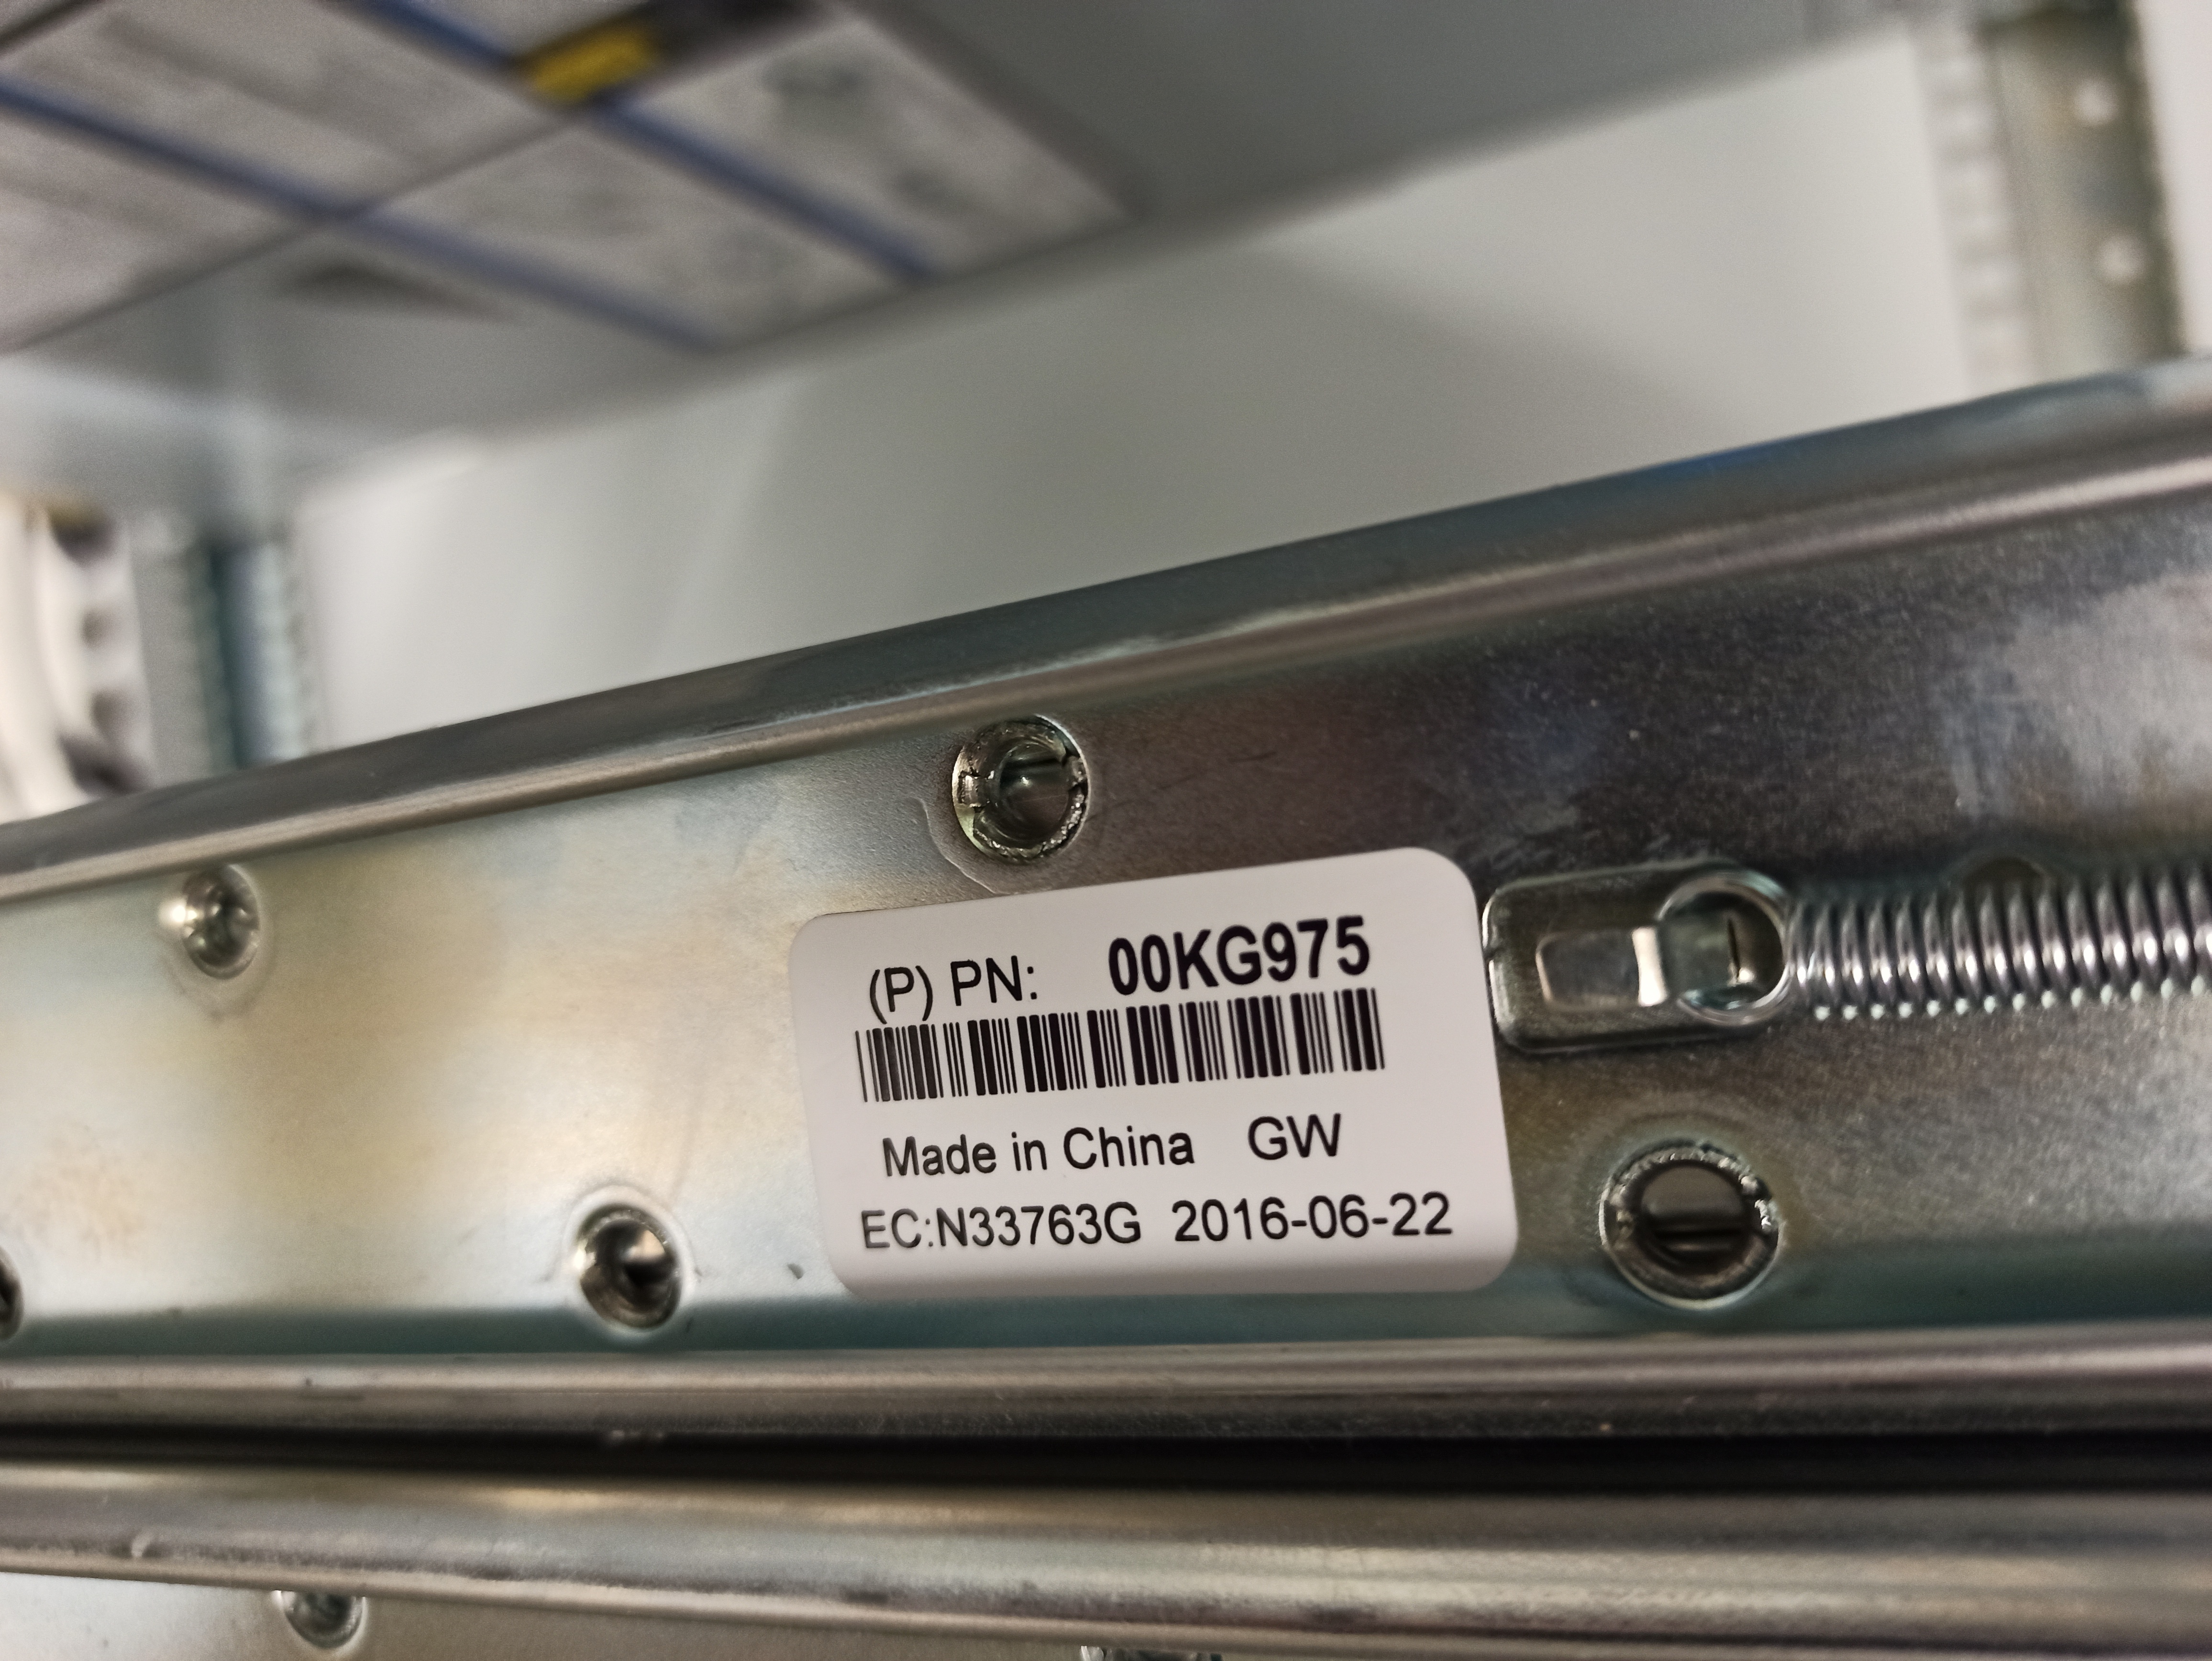
\includegraphics[width=0.40\textwidth]
        {img/Image-Example-Positive.jpg}}
    \subfigure[Negative example\label{fig:bad-example}]{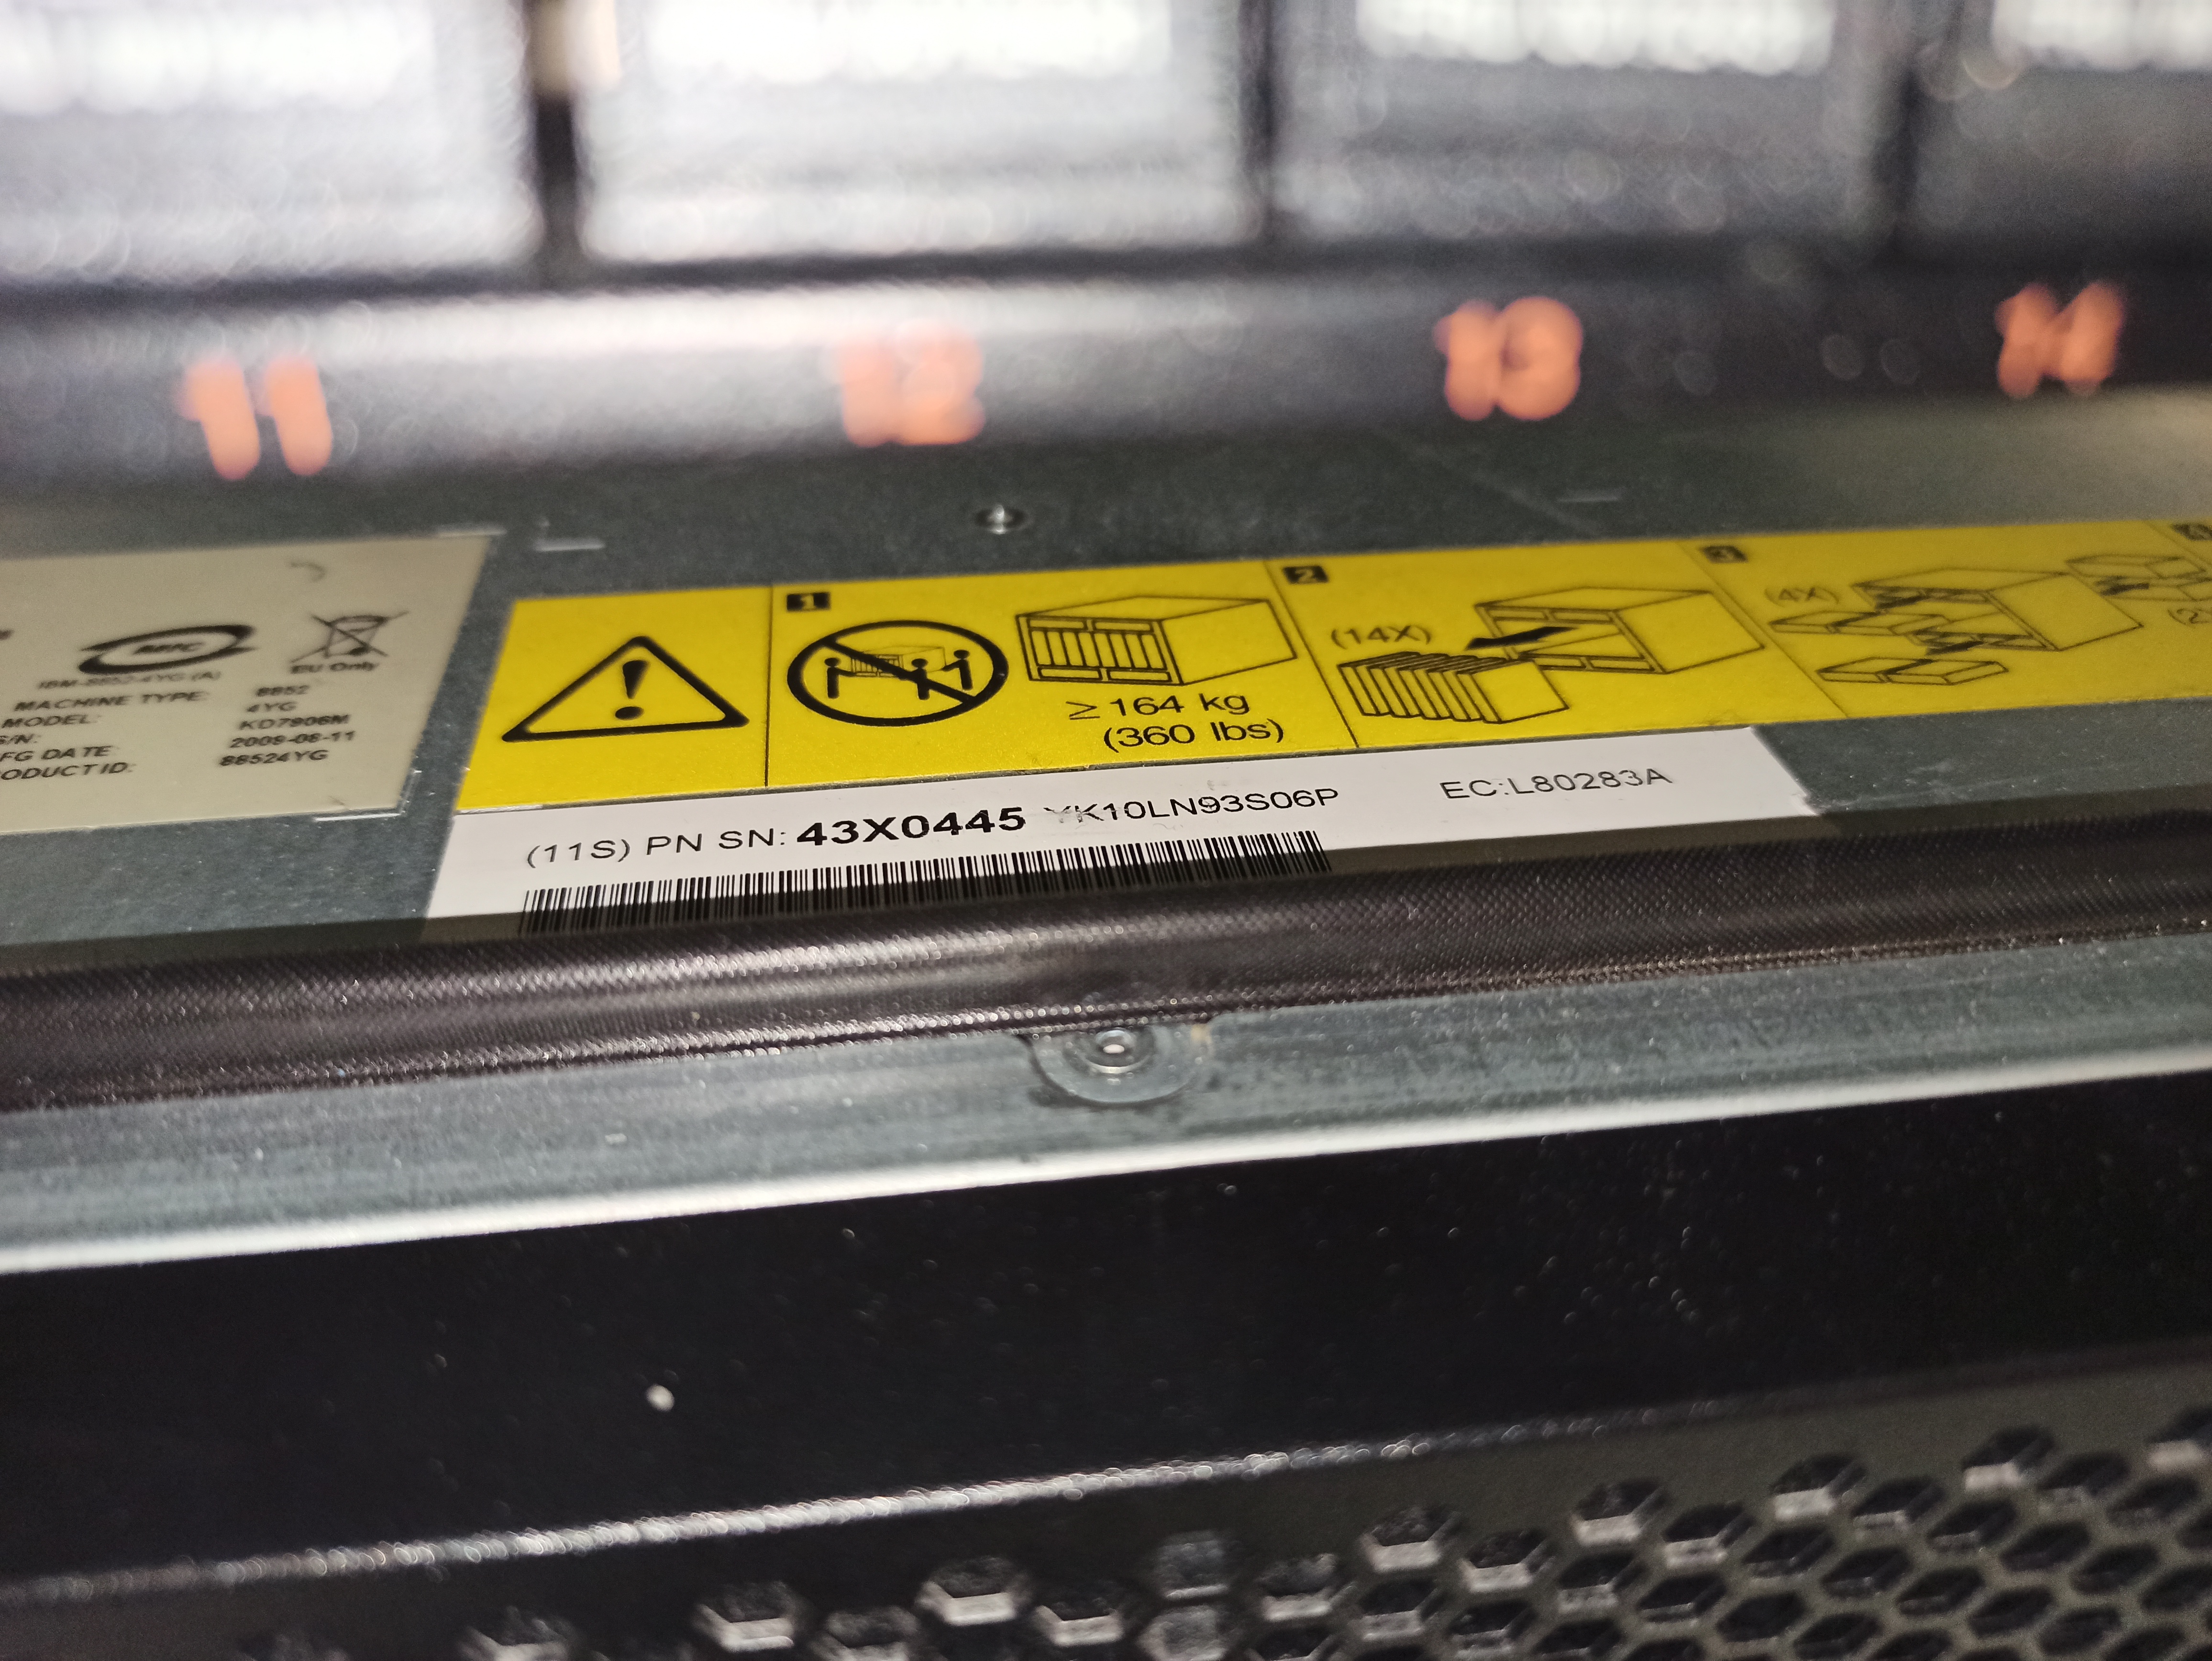
\includegraphics[width=0.40\textwidth]
        {img/Image-Example-Negative.jpg}}
    \caption{Examples for label images\label{fig:examples}}
\end{figure}
% XXX: use concept of representation for semantics retention
The text, spacing and structure carries semantic information which can be important for later
processing in the scope of a business process~\citep{chen_text_2021}.
The goal is to extract the text and preserve semantics from structure and space.
This means text and the respective coordinates, height, width and a possible rotation angle must
be output as the result~\citep{yang_learning_2021}.
Those values can then be transformed into other formats such as JSON or HTML as needed.
The labels can contain arbitrary alphanumeric strings such as serial numbers (see
figure~\ref{fig:examples}).
This results in the requirement that the \ac{DL} model has to be able to recognize sequences that
are not part of a predefined lexicon~\citep{ghosh_visual_2017}.
The qualities for the \ac{MLS} that can be derived directly from the use case (see
table~\ref{tb:literatureQualities}) can be regarded as excluding criterias, because an approach
that does not possess the qualities in question, cannot be regarded as viable for the use case.
\begin{table}[h]
    \centering
    \begin{tabular}{l c}
        Alphanumeric recognition    & Recognize alphanumeric strings such as serial \\
                                    & numbers \\
        Semantics retention & Retain semantics given implicitly be space, \\
                            & strucure and rotation of text in labels \\
    \end{tabular}
    \caption{Qualities specific to use case --- exclusion criterias}
\end{table}

In addition to the qualities that arise directly from the use case, literature reveals a number of
common qualities in regards to \ac{MLS} (see table~\ref{tb:literatureQualities}), some of which
can be regarded as relevant and other do not hold any relevance for the specific use case.
The qualities are taken from literature which covers \ac{ML} in general to literature
which covers \ac{STR}.
Only qualities that concern the model will be looked at because the model is the focus of this thesis.
These qualities may however be influenced by other entities.

% FIXME: some can be quantified, some can't

\begin{table}[h]\label{tb:literatureQualities}
    \centering
    \begin{tabular}{c c}
        Relevant                & Not relevant \\
        \hline
        Performance & Interpretability (ashmore, siebert) \\
        Robustness & Reusability (ashmore) \\
        Performance efficiency (zhang, El Bahi)  & Security / Data protection (Siebert, zhang)\\
        Appropriateness & Fairness (siebert, zhang) \\
                                & Maintainability \\
    \end{tabular}
    \caption{Qualities identified through literature}
\end{table}
% TODO: qualities often under different name -> also name source and explain?

% Performance
% FIXME: explain relevence
`An ML model is performant if it operates as expected according to a measure (or set of measures)
that captures relevant characteristics of the model output'~\citep{ashmore_assuring_2021}.
The measure is chosen depending on the type of task to be solved~\citep{siebert_construction_2021}.
The F-Score is an example for a metric that is used to compare different
models~\cite{chen_text_2021, long_scene_2021}.
Performance is usually measured with a test dataset that is independed from training and validating
a model~\cite{goodfellow_deep_2016}.
% FIXME: combine from \cite{siebert_construction_2021}: Correctness, appropriateness, Relevance
% FIXME: from \cite{nakamichi_requirements-driven_2020}: generalization performance, sufficiency of
%        accuracy

% Robustness
% FIXME: focus from literature
The robustness of a model concerns environmental uncertainty~\cite{ashmore_assuring_2021}.
Due to the uncontrolled environment of \ac{STR} in the practical aspect of taking the images on-site
beneficial image properties can not be guaranteed~\citep{chen_text_2021}.
Robust text extraction can be influenced by factors such as complex backgrounds, text form
(text rotation, font variability, arrangement), image noise (lighting conditions, blur,
interference and low resolution) and access (perspective, shape of
text)~\citep{oyedotun_deep_2015,ghosh_visual_2017,chen_text_2021}.
Therefore, these properties have to be accounted for when determining the viability for an approach.
An example for bad image quality in regards to \ac{OCR} can be seen in figure~\ref{fig:bad-example}.

% FIXME: revisit \cite{hu_towards_2020} for definition of transformations (invariant, equivariant)
% FIXME: e.g. add gaussian noise, rotate stuff, ...

% FIXME: work in following notes:
`Increasing model complexity generally reduces training errors, but noise in the training data may result in overfitting and in a failure of the model to generalise to real-world
data'~\citep{ashmore_assuring_2021}.
Aspect ratios and perspective distortions~\cite{sourvanos_challenges_2018}
`Perspective distortion is an inherent issue when the optical axis of the camera is not perpendicular to the text plane. Shapes of characters are distorted, skewed or stretched.'~\cite{sourvanos_challenges_2018}

% Appropriateness (sieber, nakamichi)
Whether model type is appropriate for the task~\cite{nakamichi_requirements-driven_2020}
Degree to which model type is appropriate for current task and can deal with current data
type~\cite{siebert_construction_2021}

% Interpretability (ashmore, siebert)
extent to which model can produce artefacts that support the analysis of its output~\citep{ashmore}
`Interpretable models aid assurance by providing evidence that allows for [2, 96, 99]: justifying the results provided by a model, supporting the identification and correction of errors, aiding model improvement, and providing insight with respect to the operational domain.'~\citep{ashmore_assuring_2021}
`The difficulty of providing interpretable models stems from the frequent use of complex ML models whose structure and size makes it impossible for a human to construct a mental model that can explain the features and parameters of the model in a contextually meaningful manner.'~\citep{ashmore_assuring_2021}
degree to which trained model can be interpreted by humans~\cite{siebert_construction_2021}

Explainability twofold: explain the model (what has been learned) explain single preditictions of the model~\cite{vogelsang_requirements_2019}

modular processing pipeline replaced with large NN that are trained end-to-end
$\rightarrow$ trade transparency for accuracy~\cite{arpteg_software_2018}

% Reusability (ashmore)
Ability of model to be reused in systems for which not originally intended $\rightarrow$ reuse of
pre-trained model for transfer learning~\citep{ashmore_assuring_2021}

% how well do overviews transfer to given dataset?


% Performance efficiency (zhang, El Bahi, Siebert)
Resource utilization when already trained~\citep{siebert_construction_2021}
The computational power of smartphones demonstrates large variations, which depend on the
smartphone model.~\cite{sourvanos_challenges_2018}
`Especially for vision-based applications, such as OCR, computational complexity is a key factor, as can be noticed for other applications of visual computing in mobile devices [18]. Apart from more technical requirements, such as a de- cent camera, processing of multimedia information on mobile devices in interactive or real time is either computationally demanding (which results in high power consumption, bad performance of other functions, etc.) or cannot be done at all.'~\cite{sourvanos_challenges_2018}
time behaviour and resource utilization (data storage)\cite{nakamichi_requirements-driven_2020}

Resource limitations> lack of memory, long training time, low-latency needs~\cite{arpteg_software_2018}


% Security / Data protection (Siebert, zhang)
GDPR:\ personal data can only be used in ways specified by explicit consent~\cite{vogelsang_requirements_2019}
security, safety, data protection~\cite{siebert_construction_2021}
% Fairness (siebert, zhang)
ability to output fair decisions~\cite{siebert_construction_2021}
also: freedom from discrimination, problem with \ac{MLS}: discrimination is implicit, \ac{MLS} amplify
discrimination bias in the data~\cite{vogelsang_requirements_2019}
% Maintainability (Nakamichi)
Modifiability (resource or software update), Analyzability (System Status
analysis)~\cite{nakamichi_requirements-driven_2020}
`Version control for ML systems adds a number of challenges compared to traditional software
development, especially given the high level of data dependency in ML
systems.'~\cite{arpteg_software_2018}
`With the addition of data dependencies and a high degree of configuration parameters, it can
be very challenging to properly maintain ML systems in the long run. Also, it is not uncommon to
perform hyperparameter tuning of models, potentially by making use of automated meta-optimization
methods that generate hundreds of versions of the same data and model but with different
configuration parameters [35]. Deep learning can also add the requirement of specific hard-
ware.'~\cite{arpteg_software_2018}

\chapter{Technique Overview}\label{ch:research}
This part of the thesis constitutes the main part.
The objective is to create an overview of techniques in the field which may be used to solve the
problem detailed in Chapter~\ref{ch:problem}.
First the search for literature which lays the foundation for the subsequent sections, is documented.
The a taxonomy is introduced which facilitates the analysis and comparison of techniques.
Lastly, the advances in the field are placed in the correct position and analyzed.

\section{Taxonomy of Pipeline Steps}
In order to create the overview the necessary steps in the process of \ac{STS} need to be highlighted,
from preprocessing to classifying the identified
text~\citep{long_scene_2021, sourvanos_challenges_2018}.
The ways in which the respective issues for the steps are solved are identified from literature,
listed and explained alongside.
\begin{figure}[h]
    \centering
    \resizebox{0.8\linewidth}{!}{%
\begin{tikzpicture}[
    every node/.style={draw=black,thin,anchor=west, minimum height=2.5em},
    lroot/.style={%
        edge from parent fork down,
        level distance=0.5cm,
        text centered, text width=3cm},
    lone/.style={%
        text centered, text width=3cm,
        level distance=0.5cm},
    ltwo/.style={%
        text centered, text width=3cm,
        level distance=0.5cm},
    lthree/.style={%
        rounded corners,
        grow=down, xshift=-0.8cm,
        text centered, text width=3cm,
        edge from parent path={(\tikzparentnode.205) |- (\tikzchildnode.west)}},
    level1/.style ={level distance=1.2cm},
    level2/.style ={level distance=2.4cm},
    level3/.style ={level distance=3.6cm},
    level4/.style ={level distance=4.8cm},
    level5/.style ={level distance=6.0cm},
    level 1/.style={sibling distance=8cm},
    level 1/.append style={level distance=1.5cm},
    level 2/.style={sibling distance=4cm},
    level 2/.append style={level distance=1.5cm},
]
%   \draw[help lines] (0,0) grid (4,3);

    % lroot
    \node[anchor=south,lroot]{STS}
    [edge from parent fork down]
        child{node [lone] {STD}
            child{node [ltwo] {Anchor \\ based}
                child[lthree,level1] {node {Feature \\ Extraction}}
                child[lthree,level2] {node {Text \\ localization}}
                child[lthree,level3] {node {Filter \\ results}}
            }
            child{node [ltwo] {Segmentation \\ based}
                child[lthree,level1] {node {Feature \\ Extraction}}
                child[lthree,level2] {node {Sub-components \\ segmentation}}
                child[lthree,level3] {node {Text \\ reconstruction}}
            }
        }
        %
        child{node [lone] {STR}
            child{node [ltwo] {Segmentation \\ based}
                child[lthree,level1] {node {Image \\ preprocessing}}
                child[lthree,level2] {node {Feature \\ extraction}}
                child[lthree,level3] {node {Character \\ segmentation}}
                child[lthree,level4] {node {Character \\ recognition}}
            }
            child{node [ltwo] {Segmentation \\ free}
                child[lthree,level1] {node {Image \\ preprocessing}}
                child[lthree,level2] {node {Feature \\ extraction}}
                child[lthree,level3] {node {Sequence \\ modelling}}
                child[lthree,level4] {node {Prediction}}
            }
        }
        %
        child{node [lone] {E2E}
            child{node [ltwo] {Two Stage}
                child[lthree,level1] {node {STD}}
                child[lthree,level2] {node {STR with \\ feature maps}}
            }
            child{node [ltwo] {One Stage}
                child[lthree,level1] {node {STD \& STR \\ Parallel}}
            }
        };

\end{tikzpicture}
}%


\begin{comment}
\begin{tikzpicture}[
    font=\scriptsize,
    edge from parent fork down,
    level distance=1.75cm,
    every node/.style={
            rectangle,
            minimum height=6mm,
            align=center,
            text depth = 0pt,
    },
    edge from parent/.style={draw=black},
    category/.style={Rectangle},
    step/.style={Circle}
]
    \Tree [.STS
        [.{STD}
            [.{Feature \\ Extraction} ]
            [.{BB Regression} ]
        ]
        [.{STR}
            [.{Preprocessing} ]
            [.{Feature \\ Extraction} ]
            [.{Sequence \\ Modelling} ]
            [.{Prediction} ]
        ]
    ]
\end{tikzpicture}
\end{comment}

\caption{Pipeline taxonomy and respective steps\label{fig:pipelineSteps}}
\end{figure}
Figure~\ref{fig:pipelineSteps} shows tasks which are associated with \ac{STS}.
\ac{STD} and \ac{STR} only incorporate a part of \ac{STS}, while E2E
incorporate both \ac{STD} and \ac{STR} techniques to solve \ac{STS}~\citep{long_scene_2021}.
Therefore this section will first discuss the two parts, to then combine them.

For \ac{STD} two main categories of approaches can be identified: segmentation based and anchor
based~\citep{long_scene_2021,sheng_centripetaltext_2021,liu_accurate_2020}.
% FIXME: anchor based can also be regression based -> change to BB regression
% FIXME: check whether convolutional predictor always has softmax!!!
The anchor based category draws heavy inspiration from the field of object
detection~\citep{long_scene_2021,liu_accurate_2020}.
This is only natural as text detection can be seen as a type of object
detection~\citep{liu_accurate_2020,long_scene_2021}.
For object detection inspired \ac{STD} there are two methods: one stage and two
stage~\citep{long_scene_2021}.
% FIXME: why one / two
Both localize text instances as a whole~\citep{long_scene_2021,sheng_centripetaltext_2021}.
One stage approaches are modelled after~\cite{liu_ssd_2016}, Single Shot MultiBox
Detector (SSD) and~\cite{redmon_you_2016}, You Only Look Once (YOLO).
\begin{figure}[ht]
    \centering
    \includegraphics[width=0.8\textwidth]{img/STD-seg-free-Liao-TextBoxes-2017.png}
    \caption[One stage, anchor based STD architecture]{Example for a one stage, anchor based STD
    architecture~\citep{liao_textboxes_2017}\label{fig:STD-segfree-ssd}}
\end{figure}
The basic approach is explained with the example of~\cite{liao_textboxes_2017} (see
Figure~\ref{fig:STD-segfree-ssd}) which is based on SSD.%
It uses 13 layer convolutional network (three blocks of: two or three $3\times3$ conv layers followed
by a $2\times2$ max pooling layer) for feature extraction~\citep{liao_textboxes_2017}.
Afterwards come nine additional layers which continuously downsample, the output of six of them
is separately used as feature maps for \ac{BB} regression~\citep{liao_textboxes_2017}.
The downsampling and \ac{BB} regression for different layers helps detect text instances of different
scales~\citep{liu_ssd_2016}.
Each spatial location on the feature map can be traced back to a region on the input
image~\citep{long_scene_2021}.
The \ac{BB} regression is carried out by six text-box layers which predict how certain ($c_1,c_2$)
the prediction is a text instance or background and where the text instance is ($x,y,w,h$).
Note that the output is not the location of a \ac{BB} but the offset to the
respective anchor box~\citep{liao_textboxes_2017,long_scene_2021}.
Anchor boxes are predefined to give bias towards sizes and aspect ratios of
text~\citep{liao_textboxes_2017}.
The text-box layers are the difference to the SSD approach for normal object
detection~\citep{liao_textboxes_2017,liu_ssd_2016}.
These layers use $1\times5$ filters to adjust to larger aspect ratios~\citep{liao_textboxes_2017}.
Each text-box layer has 72 filters (12 anchor boxes $\cdot$ 6 values per prediction), the filters
are slided accross the input features generating 12 predicted \ac{BB} per
position~\citep{liao_textboxes_2017}.
The \acp{BB} of all layers are then subjected to the process of \ac{NMS} to filter out the best
\ac{BB} for each possible text instance~\citep{liao_textboxes_2017}.
For this \ac{NMS} is used: of all detections which overlap more than a threshhold $\phi$ only the
with the highest confidence score ($c$) is kept~\citep{hosang_learning_2017}.

The R-CNN which builds the foundation for \ac{ROI} based text detection, was introduced
by~\cite{girshick_rich_2014} and improved by~\cite{girshick_fast_2015} (Fast
R-CNN),~\cite{ren_faster_2015} (Faster R-CNN) and~\cite{he_mask_2018} (Mask R-CNN).
Note that 2-stage methods are fully differentiable and thus end to end trainable since
Faster R-CNN (like 1-stage methods)~\citep{ren_faster_2015,long_scene_2021}.
The model introduced by~\cite{jiang_r2cnn_2017} (see Figure~\ref{fig:STD-segfree-rcnn}) uses
Faster R-CNN.%
\begin{figure}[ht]
    \centering
    \includegraphics[width=0.8\textwidth]{img/STD-seg-free-Jiang-R2CNN-2017.png}
    \caption[Two stage, anchor based STD architecture]{Example for a two stage, anchor based STD
        architecture~\citep{jiang_r2cnn_2017}\label{fig:STD-segfree-rcnn}}
\end{figure}
Like with the one stage approach, the two stage approach starts with feature extraction from the
image with a convolutional layers~\citep{jiang_r2cnn_2017}.
The generated feature map is used by a \ac{RPN}.
Like with the previously explained approach, the feature maps are used to regress the offset respective
to bounding boxes.
The bounding boxes are still axis aligned at this point~\citep{jiang_r2cnn_2017}.
In contrast to the previous SSD based approach, only one feature map is used in conjunction with
anchor box regression~\citep{jiang_r2cnn_2017}.
The \ac{RPN} from Faster R-CNN is adjusted to use smaller scale anchor boxes to adapt to
text~\citep{jiang_r2cnn_2017}.
Note that R-CNN and Fast-RCNN used the slower Sequential Search algorithm instead of an
\ac{RPN}~\citep{girshick_rich_2014,girshick_fast_2015}.
The resulting \acp{BB} are called \acp{ROI}~\citep{ren_faster_2015,jiang_r2cnn_2017}.
They are used for \ac{ROI} pooling in conjunction with the original feature maps.
This layer uses max pooling to convert the spatial features corresponding to the location of the
\ac{ROI} to a small feature map~\citep{girshick_fast_2015}.
In the case of this example, \ac{ROI} pooling is used to create three feature maps with different
aspect ratios ($7\times7, 3\times11, 11\times3$) which are concatenated for the next
step~\citep{jiang_r2cnn_2017}.
The second stage is to predict a confidence score (text, background) for each \ac{ROI} and to
refine them by regressing values ($x_1,y_1,x_2,y_2,h$) that allow for inclined boxes to account for
rotated text~\citep{jiang_r2cnn_2017}.
At last the resulting \acp{BB} are filtered by inclined \ac{NMS} which is adjusted to the
incline \ac{BB}~\citep{jiang_r2cnn_2017}.

The basis for the segmentation based methods is the fact that every part of the text instance can
be used to verify that there is text~\citep{long_scene_2021}.
Because of this, sub-text components can be detected separately and then used to re-construct a text
instance~\citep{long_scene_2021}.
Segmentation based methods can roughly be summed up in two categories: pixel based and component
based~\citep{long_scene_2021}.
Like with anchor based methods, example architectures are explained in order to describe their
categories more clearly.
The paper~\cite{deng_pixellink_2018} introduced a pixel based \ac{STD} approach.
\begin{figure}[ht]
    \centering
    \includegraphics[width=0.7\textwidth]{img/STD-seg-based-architecture-Deng-PixelLink-2018.png}
    \caption[Pixel, segmentation based STD architecture]{%
        Example for a pixel, segmentation based STD
        architecture~\citep{deng_pixellink_2018}\label{fig:STD-segbased-pixel-architecture}
    }
\end{figure}
Figure~\ref{fig:STD-segbased-pixel-architecture} shows the approch's architecture.
Figure~\ref{fig:STD-segbased-pixel-CNN} shows the \ac{CNN} structure for feature extraction
(until fc6\&7) followed by the head which either predicts text/non-text or
links~\citep{deng_pixellink_2018}.
The feature extraction structure is inspired by~\cite{long_fully_2015}.
Continuous downsampling and and combining those layers with later, upsampled layers helps
to combine coarse, higher level information with fine, lower level
information~\citep{long_fully_2015}.
The upsampling is performed with bilinear interpolation~\citep{deng_pixellink_2018}.
% FIXME: is this Conv Attention/Encoder-Decoder?
Depending on which head is used, the $1\times1$ convolution layers either have 2 or $2\cdot8$ filters.
Counted together, the model has 18 output channels~\citep{deng_pixellink_2018}.
The $1\times1$ convolution layers are also used for upsampling (deconvolution,
see~\cite{noh_learning_2015,long_fully_2015} for an in depth explanation)~\citep{deng_pixellink_2018}.
The 2 filters are used to predict text/non-text for each pixel, while the other 16 filters predict
the links~\citep{deng_pixellink_2018}.
The text/non-text head essentially performs semantic segmentation, that is to categorize each
pixel to its type~\citep{deng_pixellink_2018}.
A pixel has eight neighbors: left, left-down, left-up, right, right-down, right-up, up, down.
Each of the $2\cdot8$ filters is responsiblde for link a neighbor~\citep{deng_pixellink_2018}.
% FIXME: look into seglink (next approach)
\begin{figure}[ht]
    \centering
    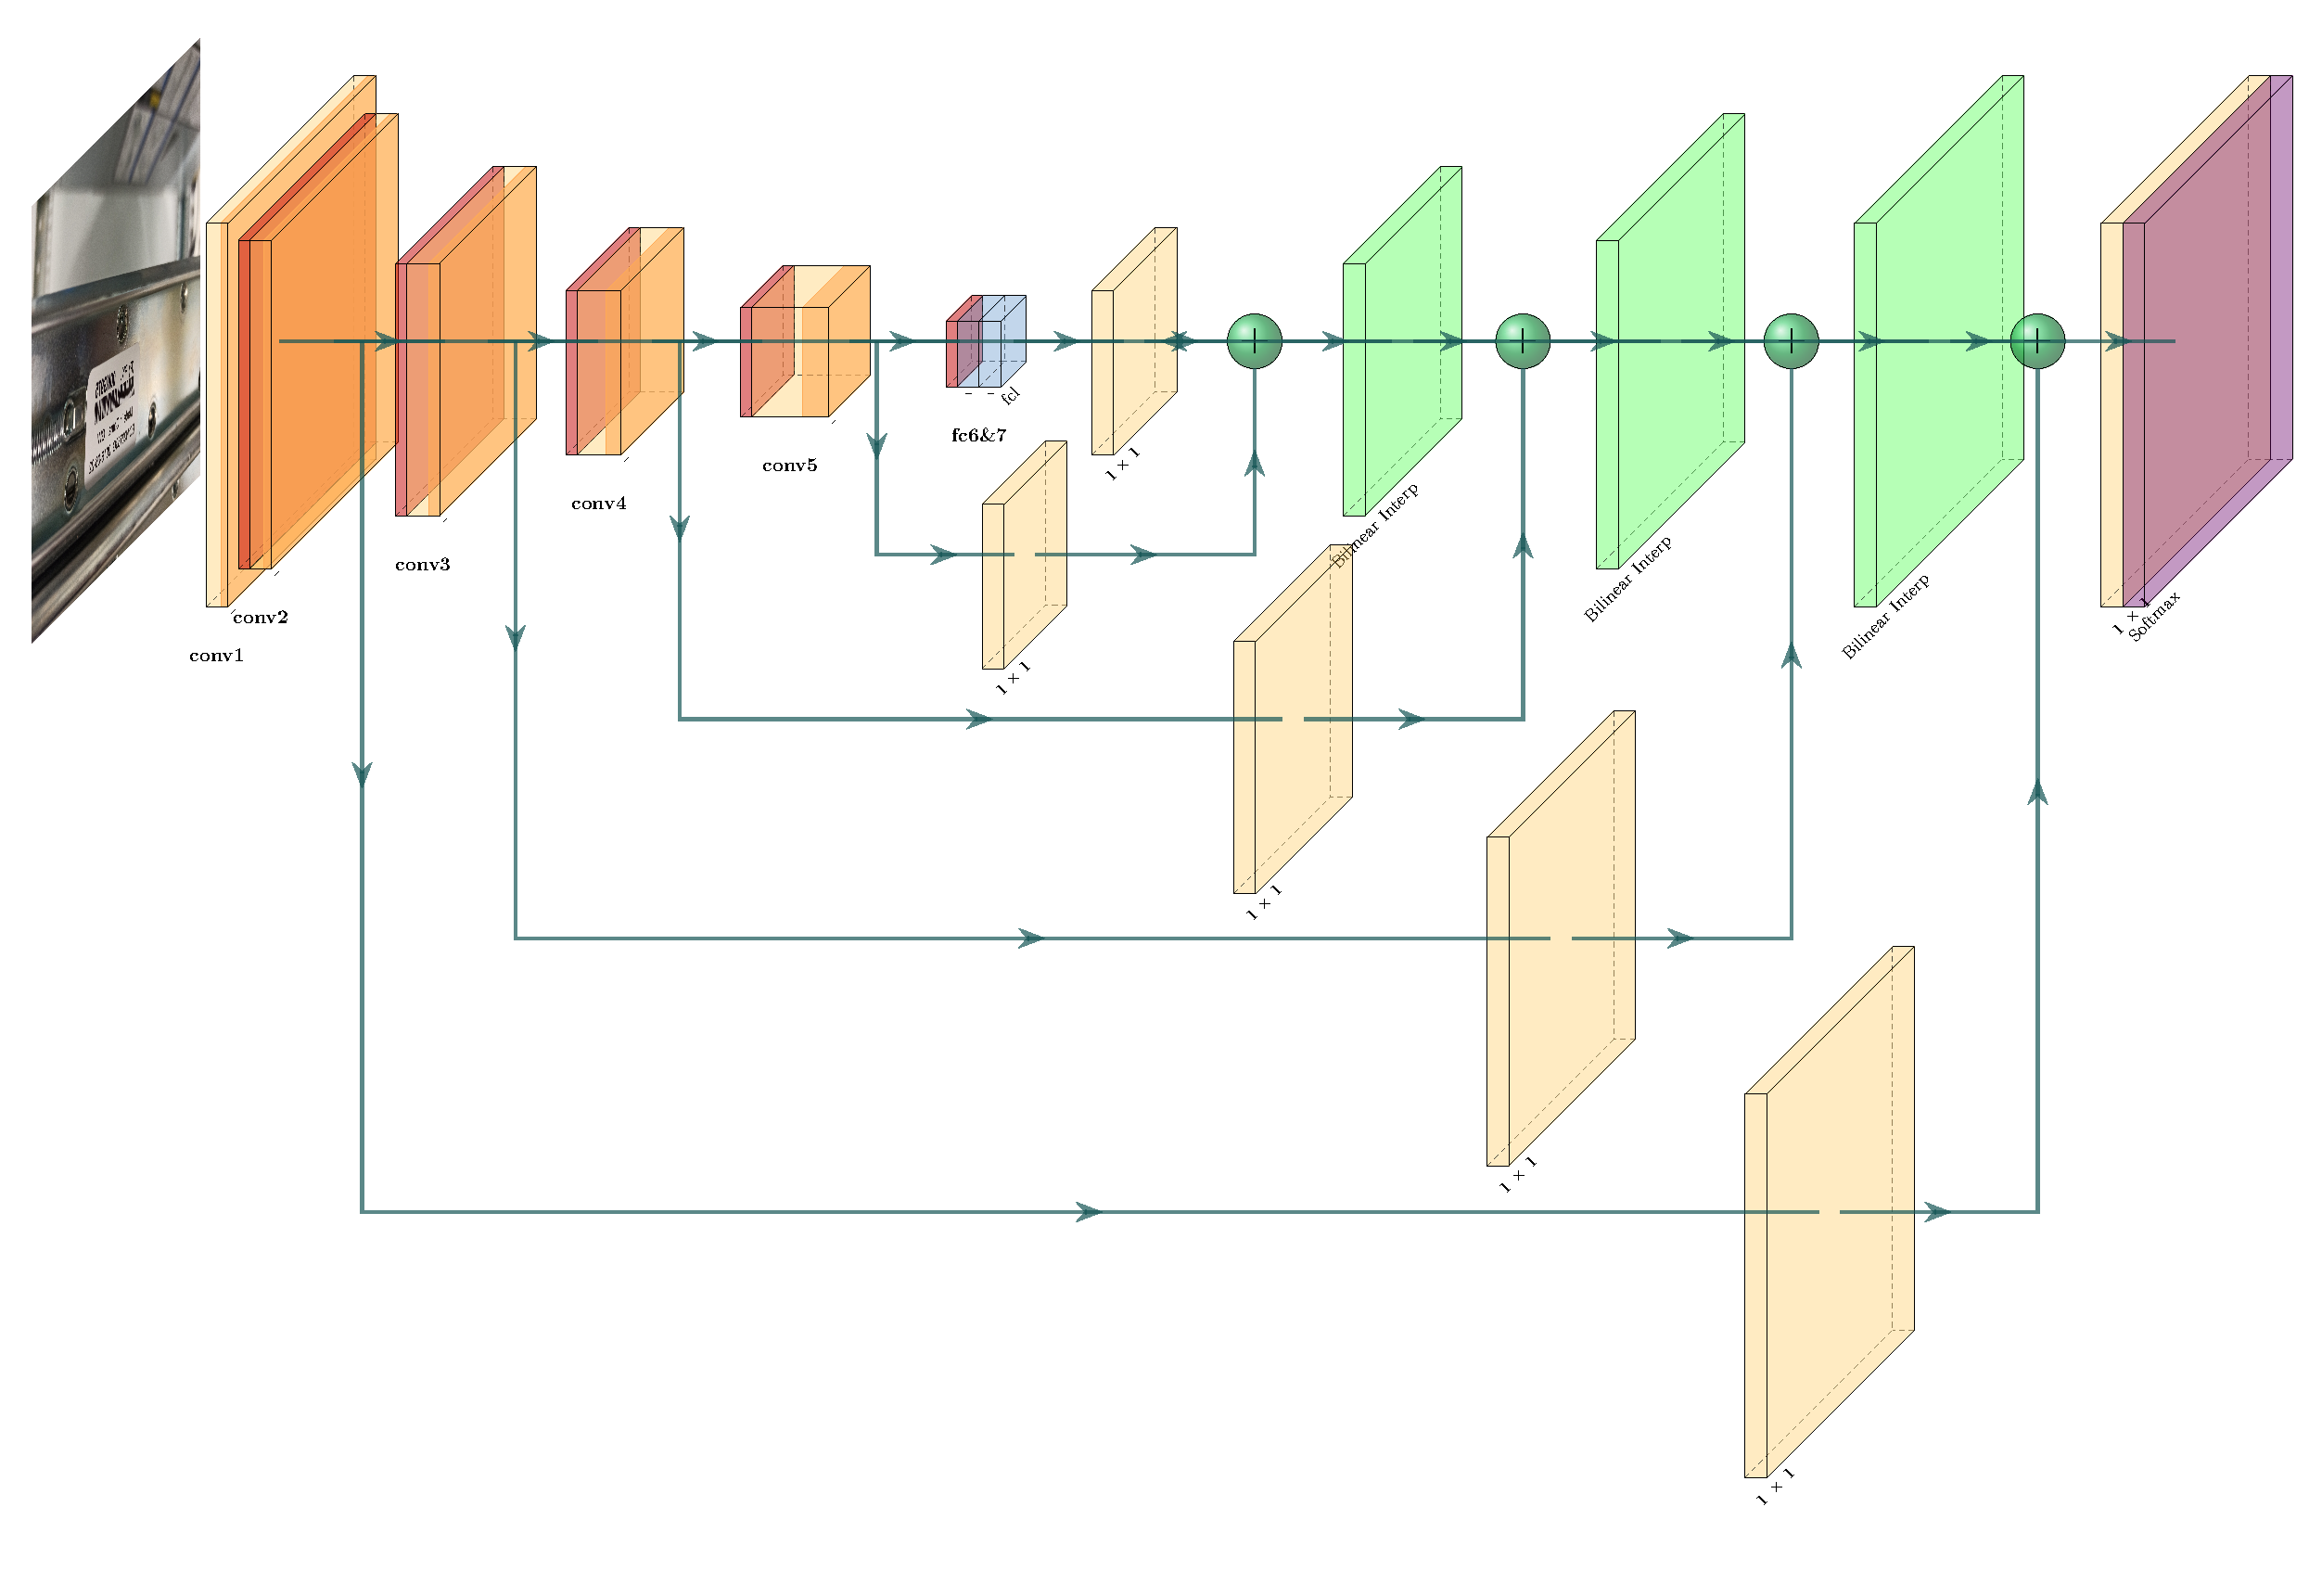
\includegraphics[width=1\textwidth]{img/STD-seg-based-CNN-Deng-PixelLink-2018.pdf}
    \caption[Feature extractor and prediction head for pixel segmentation]{%
        PixelNet CNN feature extractor with head structure for pixel
        segmentation\label{fig:STD-segbased-pixel-CNN}
    }
\end{figure}
After both links and text/non-text pixels have been predicted, they are combined for instance
segmentation~\citep{deng_pixellink_2018}.
The link layers are used to indicate whether two text pixels are grouped together an thus belong to
the same instance~\citep{deng_pixellink_2018}.
A bounding box can then be extracted by laying minimum area rectangles over the
instances~\citep{deng_pixellink_2018}.
% FIXME: final output same spatial structure as inout image

The second segmentation based category for \ac{STD} segments components which are local regions of
text that can overlap one or more characters~\citep{long_scene_2021}.
\begin{figure}[ht]
    \centering
    \includegraphics[width=0.9\textwidth]{img/STD-seg-based-architecture-Shi-Detecting-2017.png}
    \caption[Sub-component, segmentation based STD architecture]{%
        Example for a sub-component, segmentation based STD
        architecture~\citep{shi_detecting_2017}\label{fig:STD-segbased-component-architecture}
    }
\end{figure}
The architecture (see Figure~\ref{fig:STD-segbased-component-architecture})
from~\cite{shi_detecting_2017} is used as an example for this category.
Like the one-stage, anchor based \ac{STD} approach, the feature extraction \ac{CNN} of this approach
is taken from SSD, the difference is reflected in the prediction
layers~\citep{shi_detecting_2017,liu_ssd_2016}.
Instead of detecting whole \acp{BB}, the networks predicts both subcomponents and links at multiple
scales~\citep{shi_detecting_2017}.
The convolutional prediction is carried out with seven $3\times3$ filters followed by a softmax
nonlinearity for normalization.
The segments are given by the values $x_s,y_s,w_s,h_s,\theta_s$ which offset an anchor box as well
as confidence scores $c_1,c_2$~\citep{shi_detecting_2017}.
Links are used to separate the segments and are accordingly used to separate neraby
words~\citep{shi_detecting_2017}.
% FIXME: how exactly is link predicted --- conv or this calc?
Within layer links are predicted by $2\cdot$ for the neighbors of a space in the feature map
(see Figure~\ref{fig:STD-segbased-component-links} (a),
Equation~\ref{eq:STD-segbased-subcomp-same-layer})~\citep{shi_detecting_2017}.
\begin{equation}\label{eq:STD-segbased-subcomp-same-layer}
    \mathcal{N}_{s^{x,y,l}}^w =
        \frac{{\{s^(x',y',l)\}}_{x-1\leq x'\leq x+1,y-1\leq y'\leq y+1}}{s^{(x,y,l)}}
\end{equation}
The cross layer links on the other hand are predicted by using the 4 cross layer neighors of the
feature map of the preceding predictor~\citep{shi_detecting_2017}.
(see Figure~\ref{fig:STD-segbased-component-links} (b),
Equation~\ref{eq:STD-segbased-subcomp-cross-layer})~\citep{shi_detecting_2017}.
\begin{equation}\label{eq:STD-segbased-subcomp-cross-layer}
    \mathcal{N}_{s^{x,y,l}}^c = {\{s^{(x',y',l-1)}\}}_{2x\leq x'\leq 2x+1,2y\leq y'\leq 2y+1}
\end{equation}

\begin{figure}[ht]
    \centering
    \includegraphics[width=0.5\textwidth]{img/STD-seg-based-links-Shi-Detecting-2017.png}
    \caption[Predicting links for segmentation based STD]{%
        Visualization for prediction of links within and cross layers for segmentation based
        STD\label{fig:STD-segbased-component-links}
    }
\end{figure}

\begin{itemize}
    \item Links: connect segments and separate nearby instances
        \begin{itemize}
            \item within layer: connect on same layer
            \item cross layer: connect between layers
        \end{itemize}
    \item use within and cross layer links to connect adjacent locations, scales
    \item Find whole instance by depths-first search
\end{itemize}

% FIXME: after all explained: Note that mixtures of the categories are possible in practice,
%           the categorization is applied to help compare approaches (give example for mixture)

STR
\begin{itemize}
    \item segmentation-free approach (segmentation-based implicit and explicit out of date)
    \item Steps: Preprocessing, Feature Extraction, Sequence Modelling, Prediction
    \item preprocessing, text enhancement: remove distortions, background; improve resolution,
        recover degraded text
        \begin{itemize}
            \item Spatial Transformer Networks (for distortions)
        \end{itemize}
    \item feature extraction: encode image into feature space
        \begin{itemize}
            \item ResNet
                \begin{itemize}
                    \item aggressive downsampling
                    \item $3\times3$ best kernel size
                    \item Gradient saving $\rightarrow$ Res block, Res Bottleneck, Res Grouped
                    \item batch normalization
                    \item 32,50,150,\ldots
                \end{itemize}
            \item GoogLeNet
        \end{itemize}
    \item Sequence and Prediction
        \begin{itemize}
            \item CTC
            \item Encode-Decoder/Attention
            \item Lexicon Free Models!
        \end{itemize}
\end{itemize}

E2E
\begin{itemize}
    \item trainable as one?
    \item Bestandteile nicht zwangsweise sequentiell
    \item two step or two stage pipeline
\end{itemize}

\begin{table}[ht]
    \centering\scriptsize
    \begin{tabular}{p{.05\textwidth}p{.1\textwidth}p{.15\textwidth}p{.55\textwidth}}
        Task & \multicolumn{2}{c}{Approach} & Identifying properties \\
        \toprule
        STD & Seg free & & Localize text instance whole \\
            & & 1-stage & direct \ac{BB} regression \\
            & & 2-stage & find \acp{ROI}, adjust \acp{ROI} for better fit \\
            & Seg based & & Localize sub text components \\
            & & Pixel-level & Pixel level segmentation \\
            & & Component-level & Sub-component level segmentation \\
        \midrule
        STR & Seg based & & Character segmentation and classification\\
            & Seg free & & Text instance recognition \\
            & & CTC based &  \\
            & & Attention based & Encoder-Decoder Mechanism \\
        \midrule
        E2E & 2-step & & \\
            & Parallel & & \\
        \bottomrule
    \end{tabular}
    \caption{Tasks, method categories and identifying propertis\label{tb:steps-properties}}
\end{table}

\section{Literature Search}\label{se:litSearch}
This section documents the search for literature which provides the content for the subsequent
overview of innovation.
For this, important pipelines and notable advances along with their properties are researched,
analysed and presented.
The literature is identified through searching in the Google Scholar database.
The search is executed with keywords such as, but not only: Deep Learning, Text Detection,
Text Recognition, Text Spotting, Scene Text, Pipeline.
% FIXME: update keywords
A criterion for further examination is an appropriate amount of citations for the piece of literature
in question.
Additionally, literature is selected through citations for and by literature which has already been
identified as important.
All research after 2018 which pertains to extracting scene text is regarded as relevant.
Standard \ac{OCR} solutions may not hold validity in practice, as the image and text conditions can
vary in the defined problem~\citep{chen_text_2021}.
The delimination from Section~\ref{se:problem} of course holds for this chapter and only literature
which concerns advances for the \ac{DL} model architecture will be regarded as important for the
scope of this thesis.
This extends to the whole pipeline from preprocessing an image to the final result of the model.

% FIXME: hierarchical graphic with found papers
% FIXME: describe proceeding


\section{State of the Art Methods}

text enhancement:~\cite{chen_text_2021}
model pruning:~\cite{niu_26ms_2019}
integer inference:~\cite{ignatov_ai_2019}

\chapter{Discussion}
\section{Results}
\section{Method reflection}
\section{Future and follow up research}

\chapter{Conclusion}

\begin{itemize}
    \item~\cite{watanabe_preliminary_2019}:next steps to practically solve problem
        $\rightarrow$  Data Collection, Data Cleaning, Data Labeling, Model Training,
        Model Evaluation, Model Deployment, Model Monitoring
    \item~\cite{zhao_improving_2020}: Use Neural Architecture Search to automatically find right
        feature extractor
    \item~\cite{siebert_construction_2021,nakamichi_requirements-driven_2020}: build system around
        model $\rightarrow$ e.g.\ supervision mechanism
    \item~\cite{shi_icdar2017_2017,he_icpr2018_2018}: adjust field to better metrics for evaluation
    \item~\cite{long_scene_2021}: general trend to move towards simpler,shorter pipeline
\end{itemize}


% Literaturverzeichnis
%\bibliographystyle{dbstmpl}    % verwendet dbstmpl.bst
%\bibliographystyle{alpha}
\bibliographystyle{plainnat}
\bibliography{dbstmpl}          % verwendet dbstmpl.bib

\appendix
\chapter{References}
\end{document}
